\chapter{Hardware}

\begin{figure}
	\centering
	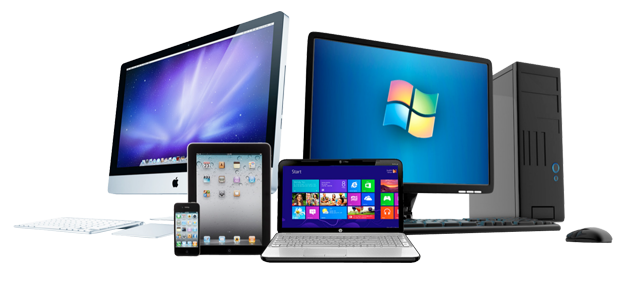
\includegraphics[width=0.85\textwidth]{images/computer_system.png}
	\caption{A variety of computer systems: desktops, a laptop, a tablet, and a
    smart phone. \afm{Source for pic.}}
	\label{fig:hardware:computers}
\end{figure}

Today's lecture will focus on \emph{computer systems} \afm{should we change the title
  to systems, this is funky to say the chapter is hardware, and then say we
  focus on systems}, groupings of devices that work together to perform a common
task (or tasks).  When most of us think about
computers, we often think of a desktop or laptop computer, equipped with a
keyboard, mouse, and monitor as seen in Figure~\ref{fig:hardware:computers}.
However, many things we interact with daily are computerized, including cell
phones, cars, traffic lights, smart watches, televisions, and manufacturing
lines. Today each of these items has sensors to perceive the real world, uses an
embedded computing device to understand the sensory input, and uses a combination
of display and mechanical devices to interact with the real world.

\begin{example}
  For intersections across busy roadways, some traffic lights are computerized
  to optimize road traffic. These lights will stay green along the busier of the
  two roads, and use cameras or pressure sensors to detect the presence of cars
  along the less busy of the two roads. When cars arrive, the lights switch,
  allowing the cars on the less busy road to cross.
\end{example}

Today we will introduce three fundamental parts of computer systems:
input and output devices, memory, and the central processing unit (CPU).
These components work together to perform the basic building blocks of
input processing, storage, control, and output. Understanding how the
three parts work together will allow us to create powerful information
processing tools. We will introduce each of these parts in turn.
In Figure~\ref{fig:hardware:overview}, we see how these parts come
together to form a computer system.

\begin{figure}
	\centering
	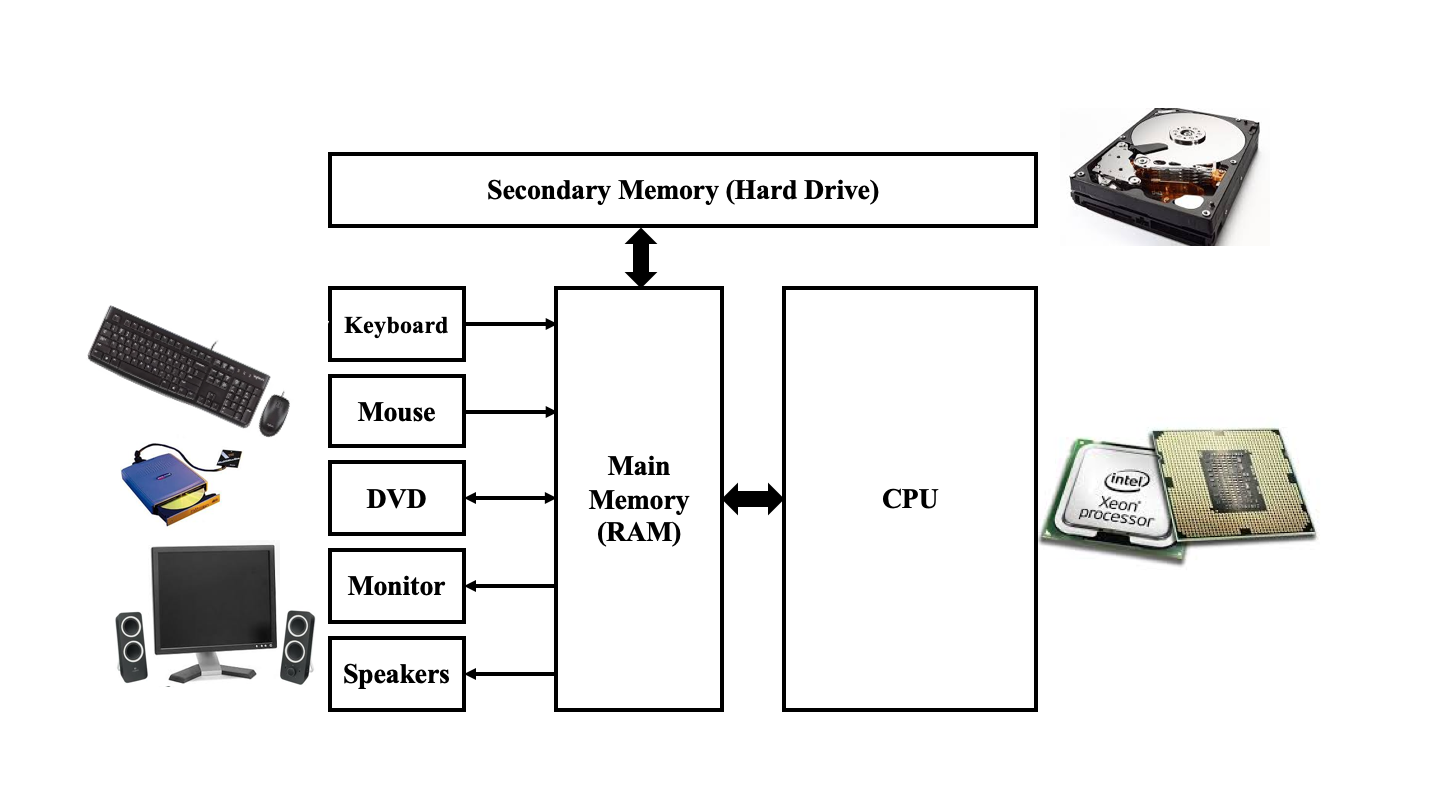
\includegraphics[width=0.85\textwidth]{images/cs_intro_hardware_overview.png}
	\caption{Interconnected parts of a computer system (keyboard, mouse,
                 monitor, DVD player / burner, speaker, hard drive, CPU).
                 \afm{source for pic}}
	\label{fig:hardware:overview}
\end{figure}

\section{Input and Output Devices}

Input and output  devices allow the computer to interact with users and the world
directly.  \emph{Input} devices are used to bring data into the computer system. Examples include keyboards, mice, and microphones. \emph{Output} devices are used to display the results or information of a computer system. The most common forms of output are words, numbers, and graphics.  Examples of output devices include speakers, printers, and monitors. With input and output devices, a
user's input will be processed, some computations will be performed, and then
the resulting output will be displayed to the user. Without these devices, a computer system would be very boring, always
performing the same computation each time it's used. Even if it did compute a
different value we would be unable to examine the value. A computer needs to be
able to accept input and output a result. The first computers would occupy a
large room in an office building and connect to a terminal (a keyboard and a
text screen) in another room for users to interact with. Thanks to the hard work
of electrical engineers,
computers can now fit in the palm of your hand while being much more powerful.
Likewise, many more types of input and output devices are now available. We
still have the keyboard and monitor, and the mouse was invented for interacting
with graphical displays. Today's phones are more computer than phone, coming
equipped with speakers, microphones, touch screens, cameras, fingerprint
scanners, radio transmitters, and much more. Computers even come embedded in
other devices like cars, traffic lights, X-ray machines, and thermostats to both
control and monitor the devices. As shown in Figure~\ref{fig:hardware:overview},
these devices connect to the rest of the computer through the computer's memory.
This kind of input and output is called memory mapped I/O (input and output).
Creators of input (or output) devices are assigned a section of the computer’s memory to write (for input devices) or read (for output devices) data. For example, a keyboard might write data about each key that is pressed to a given location. The computer will then read the data in that location to communicate with the keyboard. In the case of an output device, the process works in reverse: the computer writes the data in the assigned location, which the output device then reads. The creators of these devices agree on a known format to read and write data.

\begin{example}
  You can think of communication between devices and computer as similar to
  leaving messages for a friend in a locker. Only you and your friend have
  access to this locker, which only holds space for one message. The format you
  agree upon is which language you'll use to speak (e.g. English) and any
  special keywords or phrases. For example, you might agree upon a convention
  like the kind used in radio communication, where one person waits until they
  get an ``Over'' signal before responding with a new message.
\end {example}

The format that devices and computers communicate in are generally very simple
and structured to permit fast and easily understandable communication for
computers and devices.

\begin{example}
A monitor is a graphical display for computers. Let's consider a monitor
connected to a computer that only displays in black and white images
that are 20 x 20 pixels large. The monitor and keyboard agree upon using
the following format to communicate. The format is black and white images
that are 20 x 20 pixels large. Each pixel's value is represented at 0 for
black and 1 for white. Then an image is represented as a 400 = (20 x 20) long
sequence of pixel values. The sequence is ordered left to right, top to bottom.
Now that both the monitor and computer agree upon the communication format, the
computer can write images to the section of memory dedicated to the monitor
and the monitor will read the image and display the image on its screen.
Figure~\ref{fig:hardware:monitor_image} displays an example image, a 
20 x 20 checkerboard with its encoding.

\emph{Note: While this is a simplified example, this is similar to how modern
  graphical displays communicate with computers}.
\end{example}

\begin{figure}
	\centering
        \hspace{0.5cm}
	\begin{minipage}{0.45\textwidth}
		
\includegraphics[width=0.90\textwidth]{images/checkered_image.jpg}
	\end{minipage}
        \begin{minipage}{0.45\textwidth}
		\scriptsize
\begin{verbatim}
0 1 0 1 0 1 0 1 0 1 0 1 0 1 0 1 0 1 0 1
1 0 1 0 1 0 1 0 1 0 1 0 1 0 1 0 1 0 1 0
0 1 0 1 0 1 0 1 0 1 0 1 0 1 0 1 0 1 0 1
1 0 1 0 1 0 1 0 1 0 1 0 1 0 1 0 1 0 1 0
0 1 0 1 0 1 0 1 0 1 0 1 0 1 0 1 0 1 0 1
1 0 1 0 1 0 1 0 1 0 1 0 1 0 1 0 1 0 1 0
0 1 0 1 0 1 0 1 0 1 0 1 0 1 0 1 0 1 0 1
1 0 1 0 1 0 1 0 1 0 1 0 1 0 1 0 1 0 1 0
0 1 0 1 0 1 0 1 0 1 0 1 0 1 0 1 0 1 0 1
1 0 1 0 1 0 1 0 1 0 1 0 1 0 1 0 1 0 1 0
0 1 0 1 0 1 0 1 0 1 0 1 0 1 0 1 0 1 0 1
1 0 1 0 1 0 1 0 1 0 1 0 1 0 1 0 1 0 1 0
0 1 0 1 0 1 0 1 0 1 0 1 0 1 0 1 0 1 0 1
1 0 1 0 1 0 1 0 1 0 1 0 1 0 1 0 1 0 1 0
0 1 0 1 0 1 0 1 0 1 0 1 0 1 0 1 0 1 0 1
1 0 1 0 1 0 1 0 1 0 1 0 1 0 1 0 1 0 1 0
0 1 0 1 0 1 0 1 0 1 0 1 0 1 0 1 0 1 0 1
1 0 1 0 1 0 1 0 1 0 1 0 1 0 1 0 1 0 1 0
0 1 0 1 0 1 0 1 0 1 0 1 0 1 0 1 0 1 0 1
1 0 1 0 1 0 1 0 1 0 1 0 1 0 1 0 1 0 1 0
\end{verbatim}
        \end{minipage}
	\caption{An example checkered image and its encoding --- newlines and spaces added for readability.}
	\label{fig:hardware:monitor_image}
\end{figure}

\section{Memory}

With \emph{memory}, computers gain the ability to store and recall data. This is very
similar to physical storage of items. Figure~\ref{fig:hardware:storage} shows
three storage locations --- a storage closet, a garage, and a warehouse. Each of
the three locations make a tradeoff between convenience of location and storage
capacity. The closet can contain a few things and is the same room you need it.
The garage can fit even more things and is only a walk outside (or through) your
home, and the warehouse can fit practically anything you would want to store but
you have to drive to the warehouse to pick-up or store your items. Similarly, a
computer's memory makes the same trade-offs.

There are two major types of memory, \emph{Main Memory} (RAM) and \emph{Secondary Memory},
like hard disks, solid-state drives, tape drives, and more. Main memory is \emph{volatile},
meaning that the contents of the memory is not preserved when a computer is
turned off and back on. On the other hand Secondary Memory is meant to be
\emph{persistent} or \emph{nonvolatile}, and does not go away when the computer is turned off. Main Memory
can be thought of as the ``scratch paper'' the computer uses for computations.
Computers will also use Main Memory as a conduit for communicating between the
CPU and all other parts of the computer. Main memory is closer to a garage
(where you can lose items when you turn off the lights) --- there is enough room
to fit most items you use regularly and is close enough to not worry about the
time it takes to get to the garage.

In most modern computers,
programs are treated as data. The individual instructions that combine
to form a program are stored in memory just as data is. It is the job of the
computer to properly understand if a segment of memory is data or a program.
The computer is able to fetch data from Secondary Memory to Main Memory or
persist data in Main Memory to Secondary Memory when needed. However,
this process of transferring data between Secondary and Main Memory can
cost a lot of time relative to keeping data in Main Memory only.

\begin{figure}
	\centering
	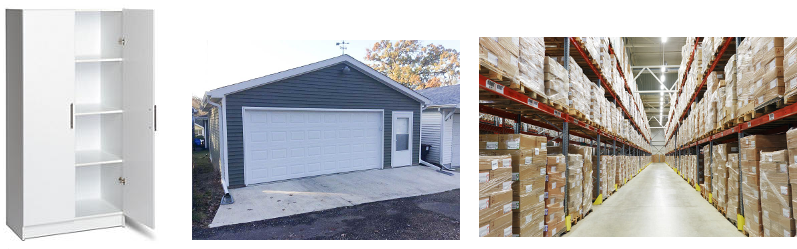
\includegraphics[width=0.85\textwidth]{images/storage.png}
	\caption{Storage closet, garage, and warehouse trading off between
                 capacity and locality. \afm{picture references}}
	\label{fig:hardware:storage}
\end{figure}

\section {Central Processing Unit}

The final part of a computer we will introduce today is the \emph{central processing
unit} (CPU), also known as the \emph{processor} or \emph{main processor}. The CPU is the physical
circuitry of a computer that performs instructions.

The CPU has several key components: the control logic, arithmetic and logic unit (ALU), registers,
program counter, and clock. These components work together to 
fetch, decode, and execute all instructions --- the building blocks of all programs.
Instructions vary between different brands of CPUs, but, in general, they will
include arithmetic, control, read (from memory), and write (to memory) functionalities.

Example~\ref{ex:hardware:instr} shows several instructions
that together would perform \ic{x = x + y}, given \ic{x} is stored in memory
location 16 and \ic{y} at memory location 20. These instructions are quite low
level, and harder for humans to read than the programs we will write in this course.
However, the programs we write will be translated into these instructions to be
easily understood and executed by the CPU.

\begin{example}
\label{ex:hardware:instr}
\begin{verbatim}
load R1 16    -- Load value at memory location 16 into register 1
load R2 20    -- load value at memory location 20 into register 2
add  R1 R2 R1 -- add the value in register 1 to the value in register 2
                 and store in register 1
store R1 16   -- store the value in register 1 to memory location 16
\end{verbatim}
\end{example}

A key component of a CPU is its clock. The clock allows the CPU to progress in time,
triggering the time to progress from time \ic{t} to time \ic{t + 1}. A single time
segment is referred to as a clock cycle. You might have heard about a computer's CPU
speed. For example, your computer may run at 2.4 GHz = 2.4 billion clock cycles per second. This
is determined by how fast the clock transitions from one time step to the next. This
clock drives the progress of the CPU. The time an instruction takes is measured
in instruction cycles. The rate of the CPU's clock is determined by the slowest
operation of the CPU.

In addition to clocks, the CPU contains a group of memory locations called registers.
A single register is capable of holding a single ``word'' of information. A ``word'' is the smallest
unit of data in a computer. The key benefit of registers is the ability for the
CPU to immediately read and write the contents of the register. The value of a register
can be updated each time the computer's clock ``ticks,'' or increments its value by one. 
Most modern CPU's will have between 16 and 64 registers that programs may use.
For comparison, accessing Main memory can take 10s or even 100s of instruction
cycles to access while registers are immediately available to the CPU.

The control unit and program counter will fetch, decode, and output the
controls for the execution of each instruction. The program counter holds the
location of the next instruction to be executed. The next instruction is then
fetched to the CPU. The CPU's control unit then decodes the fetched instruction
and outputs control signals (commands) to main memory and the ALU. The CPU may
read data from memory (e.g. store) and then the ALU will then execute the action
specified by the control unit. Example actions include add, subtract, multiply, compare to 0, etc.
The CPU may then possibly write the output to memory.

In most computers, the CPU and its constituent parts are responsible for all
computing needs of the computer. In some select systems, there will be additional
hardware to perform specialized operations (e.g. graphics processing units for
processing / producing images). It is the CPU's responsibility to control the
computer and coordinate with devices to execute programs. As such, the CPU
has seen a quick evolution to increase its processing power. Electrical
engineers originally focused on making the CPU smaller and smaller and thus
quicker. The evolution follows Moore's Law : every two years the size of a CPU shrinks
in half. Additionally, CPU's were designed with a pipelining architecture: this means
that multiple instructions are executed in quick succession. This is done
by noting that each stage of the five stages --- fetch, load,  decode, execute,
and store --- can be performed independently. Thus, while one instruction is
being executed, the next instruction can be decoded. Figure~\ref{fig:hardware:pipeline}
shows how pipelining is performed by executing the different parts of the pipeline
in parallel for five consecutive instructions.

Due to the decline of Moore's Law in recent years, many CPU designers focus on
increasing processing power by improving parallelism (i.e. being able to execute
multiple instructions at a time). This allows instructions that do not depend
on each other to be executed at the same time. These CPUs are referred to as multi-core,
as they have multiple cores that each have their own set of registers, control unit,
ALU, and program counter but share main memory and a single clock. In this class we will not
teach how to effectively harness parallel programming, but note that this is
an important progress in how hardware has evolved.

\begin{figure}
	\centering
	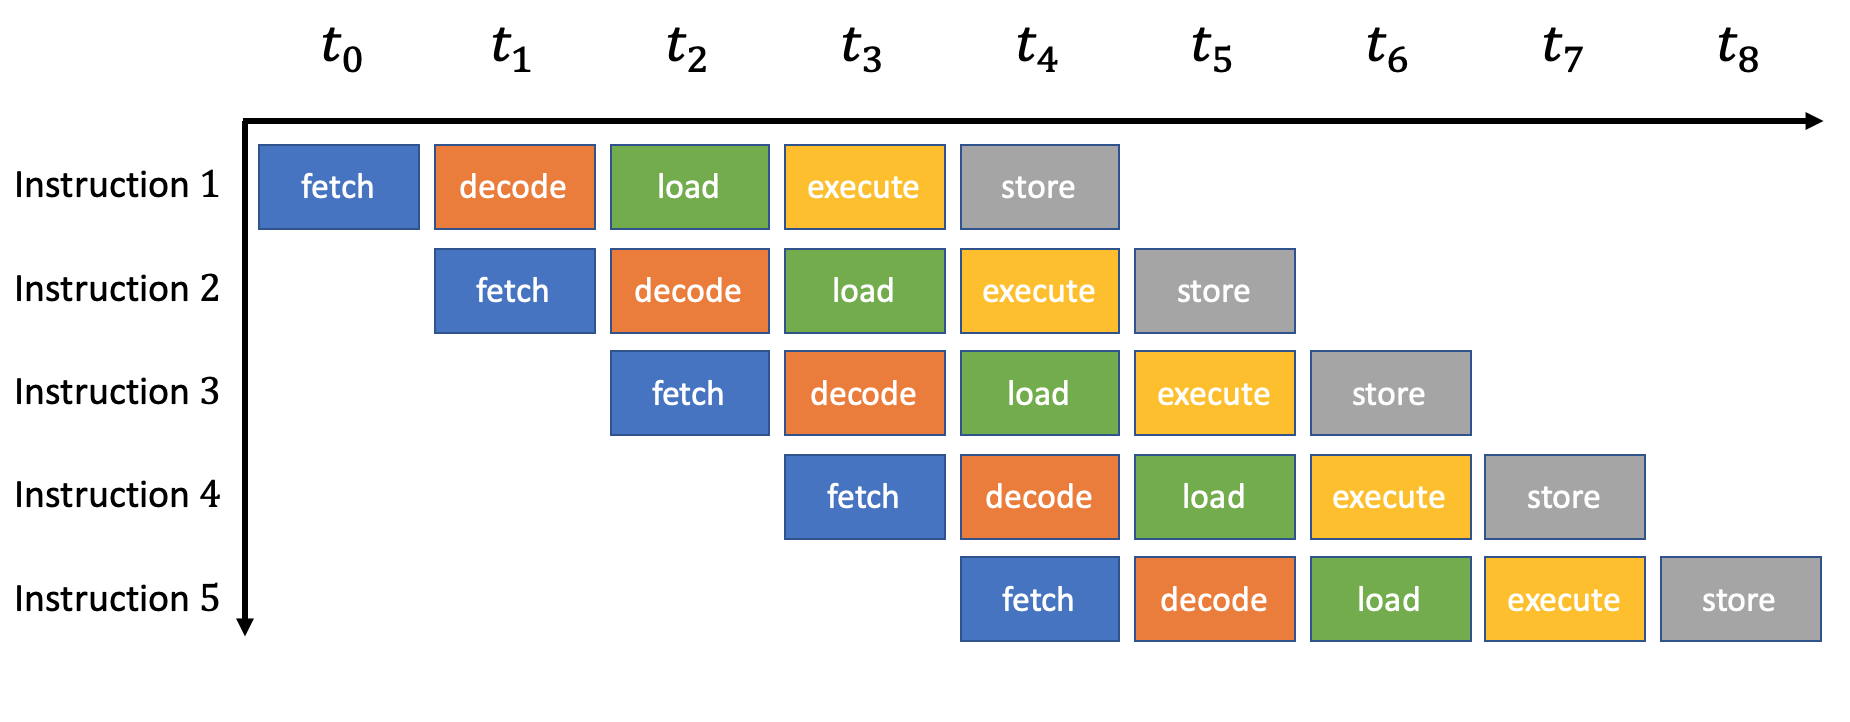
\includegraphics[width=0.85\textwidth]{images/pipeline.png}
	\caption{Instruction Pipelining. \afm{citation}}
	\label{fig:hardware:pipeline}
\end{figure}


\section {Conclusion}
In this chapter, we covered the three fundamental parts of a computer system:
input and output devices, Main and Secondary Memory, and the CPU. We discussed
their roles, relationships, and basic capabilities. We hope that this will help
you better understand how hardware works at a high level to better improve how
to write programs that will eventually run on these computer systems. In the
next chapter we will begin discussing the concept of Software and its
similarities and differences to hardware and where the boundary between the two
lies.

\exercisesection

\begin{exercise}
What three parts comprise a computer system?
\end{exercise}

\begin{exercise}
What are examples of common input and output devices?
\end{exercise}

\begin{exercise}
Name an uncommon example of a computer system and explain how it may work.
\end{exercise}

\begin{exercise}
How does memory mapped input and output work?
\end{exercise}

\begin{exercise}
Name four kinds of memory devices.
\end{exercise}

\begin{exercise}
Explain the difference between Main and Secondary Memory.
\end{exercise}

\begin{exercise}
What parts comprise the central processing unit (CPU)?
\end{exercise}

\begin{exercise}
Describe three possible methods to increase the computation power of a CPU.
\end{exercise}
